% (c) 2020 Stefan Antonowicz
% Based off of tex found at https://github.com/ludus-leonis/nipajin
% This file is released under Creative Commons Attribution-NonCommercial-ShareAlike 4.0 International License.
% Please do not apply other licenses one-way.

\renewcommand{\yggWitch}{%
  \mychapter{Witches}{witches}
}

\renewcommand{\yggWitchText}{%

  \mysection{Mojo}{witch-mojo}

  \mytable{X c r}{
    \thead{Level} & \thead{Mojo}\\
  }{
    1 & d8 \UD \\
    2-3 & d10 \UD \\
    4-5 & d12 \UD \\
    6-7 & d16 \UD \\
    8 & d20 \UD \\
    9 & d24 \UD \\
  }  

  Mojo is a \UD.  Mojo is used to cast \mylink{Charms}{witch-charms} and perform \mylink{Necromancy}{witch-necromancy}.

  When you cast Charms, you \RS your Mojo, once per Charm.  You can cast as many Charms as you like, as long as you have a Mojo \UD.

  When you perform Necromancy, you combine your Mojo \UD with your \FOC in a \RO attempt:

  \example {
    \mybold{Mojo Test}

    \RO : \mybold{Mojo \UD} plus \mybold{\FOC} plus \mybold{Modifiers}

  }

  Finally, you can use your Mojo \UD as if it were an Armor Die (see the Core Rules) if you fail your Guard \RO in Combat.

  \mysection{Cunning}{witch-cunning}

  Cunning is used to perform Occultism, and be used to help Spriggans create magic weapons.  A Cunning die is a d4; you have a base number of Cunning die equal to your \LVL (so if you were \LVL 6, you'd have 6d4 Cunning Dice).  You earn these Cunning Dice at the start of any Sabbatical you take.  Any Cunning Dice you do not use at the end of the Sabbatical are lost.

  You may obtain more Cunning Dice as specified below:

  \mytable{X X}{}
  {
    Wheel: Crown & +3 \\
    Wheel: Gibbous & +2 \\
    Wheel: Wax Quotidian & +1 \\
    Coven & +1 each member \\
    Familiar: & +1 if present \\
  }  


  You gain a Coven at 7th level (see Core Rules). 

  Cunning Dice can be traded be traded between you and other Witches. You can give as many Cunning Dice to different people as you wish, but you can only accept a number of Cunning Dice up to your \LVL-1.

  Each Occult rite requires 1 or more Cunning Dice to be rolled (how many is up to you).  You must obtain a number of successes (that is, roll a 3 or 4 on the Cunning Die) equal to or greater than what is specified in the Occult rite.  


 
  \mysection{The Wheel}{witch-the-wheel}

  Your Mojo moves counterclockwise through a Wheel of eight points - it ascends from the Void to Sickle, Quotidian, and Gibbous to Crown, then descends through Gibbous, Quotidian, and Sickle to return to the Void. 

  During character creation, roll a d8 to see where your Mojo begins:

  \mytable{l X}{}
  {
    1 & Void \\
    2 & Waning Sickle \\
    3 & Waning Quotidian \\
    4 & Waning Gibbous \\
    5 & Waxing Sickle \\
    6 & Waxing Quotidian \\
    7 & Waxing Gibbous \\
    8 & Crown \\
  }  

  Every Session, move your Mojo one step counter-clockwise along the wheel:
  \begin{center}
  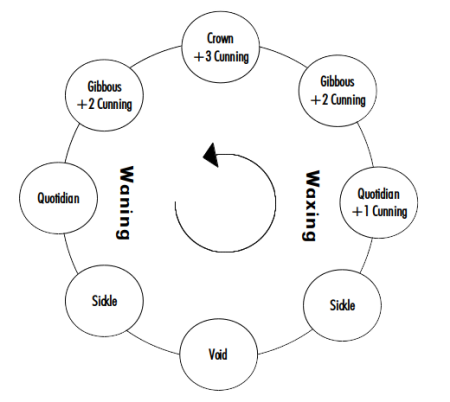
\includegraphics[scale=.3]{mojo_circle}
  \end{center}

  For some powerful rituals, you may need to move "[num] Widdershins" before you can attempt the ritual again.  A full Widdershins means you must make [num] transit(s) of the Wheel before you can cast the ritual again.  For example, if you were at Crown, you must travel to Waning Gibbous, then Waning Quotidian, etc. all the way back around to Crown before you can try again  (meaning you will need to play multiple Sessions).

  \newpage

  \mysection{Charms}{witch-charms}

  \RS with your Mojo \UD to perform a Charm.  If you smoke a bowl of pipeweed while you're casting Charms, you only fail on a 1 (instead of a 1 or 2).

  \mysubsection{Aphrodite’s Sigh}{charm-aphrodites-sigh}

  By means of this spell you can create a ghostly moaning sound that appears to come from somehere Nearby. The moan is not loud nor can it quite cause fear, but any that hear it will know of it's "unnatural" nature. 

  \mysubsection{Candlelight}{charm-candlelight}

  This spell creates a small mote of light roughly equal to candle light that hovers near your head. The spell is typically used for reading or lighting a small area (half a cubic meter). This charm cannot be cast into someone's eyes. The light is dim enough that it's not particularly useful for lighting dark passages unless that passage is very well known (such as the your own home). 

  \mysubsection{Creature Comforts}{charm-creature-comforts}

  You can raise or lower the temperature of any non-living material a few degrees, enough to warm or cool food or drinks or a room.  The temperature cannot be raised to a degree where it would injure anyone.


  \mysubsection{Dowsing)}{charm-dowsing}

  Using a forked wand of hazelwood, you can sense the direction of a substantial body of potable water.  It ignores "insignificant" amounts of water, as found in a waterskin or barrel.  The spell doesn’t tell you how hard it might be to get to the water.

  \mysubsection{Fastening}{charm-fastening}

  This spell allows you to close one door or window that is not locked or otherwise barred. This will not lock the door or window unless by the action of closing it naturally becomes locked. 

  \mysubsection{Flame of Vesta}{charm-flame-of-vesta}

  You may change a fire into one of black flame, so that it casts no light but still provides heat.  You can affect a normal fire up to the size of a campfire.  Furthermore, the flames do not burn, though they are uncomfortable to the touch.

  \mysubsection{Jinx}{charm-jinx}

  You can perform a minor hex by tracing a five pointed star in the air with your forefinger. The hex can affect something Nearby or closer.  These hexes can be severing a rope, shattering a pane of glass, spoiling a piece of food, or some other small act of malice.  Note that these hexes will not work if there is a Pooka nearby

  \mysubsection{Levitate}{charm-levitate}

  You may use this spell to lift an object via magic alone. The object needs to be non-living and weigh less than 1kg. The object will remain floating in mid-air for up to 1 Hour as long as you are paying at least some attention to it. If you are distracted at all, say in Combat or casting another spell (including another Charm) then the object drops. 

  \mysubsection{Matchstick}{charm-matchstick}

  When you drag your forefinger along a rough surface and says the name of Buer, your fingertip combusts like a giant phosphorus match. It burns for a Moment and does not hurt you in any way.

  \mysubsection{Message}{charm-message}

  By means of this spell you can send a brief message, no more than a dozen words, to a person you know. This person can be any distance away, but they have to be able to understand the language of the message you're sending.

  \mysubsection{Puff of Air}{charm-puff-of-air}

  This spell creates a small puff of air; enough to blow away dust from objects or to put out a candle, but not enough to put out a torch or lantern. The puff can move very light items as would a puff of air blown from natural means. This spell can be used to blow dirt from an item or area 1m by 1m. 

  \mysubsection{Spice}{charm-spice}

  This minor spell flavors one serving of food. The flavor can be changed but it does not change the nature of the food item nor does make poisoned food or spoiled food edible, similar to Freshen. The flavor can be chosen by you. 

  \mysubsection{Sweet Dreams}{charm-sweet-dreams}
  This spell allows you to make a willing creature fall asleep. The spell will not work if used against an unwilling subject. You can cast this spell on yourself, but this will be the last spell that you cast that day.

  If used on a subject who is already asleep, you can breathe in their ear and control what dreams they have the following night. No matter how unpleasant the dreams, this cannot prevent the victim from getting a full night’s rest on its own, but it can affect their mood.

  \mysubsection{Third Eye}{charm-third-eye}

  By holding or touching an inanimate object and concentrating for Minutes, you can detect whether or not something is magical in nature, or if something can "hold" an enchantment (including staves, swords, and holy relics).  

  Alternately, you can use this charm to "see" any Nearby concealed objects, like secret doors and hidden compartments.  The Charm doesn't detect invisible or magically concealed objects. 


  \mysubsection{Tidy}{charm-tidy}

  This spell can be used to clean a single object. The object can be anything, clothing, armor, weapons or even a area of a home. Unlike other Charms this one can be cast on a willing living participant. A warlock casting clean on themselves will appear as they would if they had recently bathed and donned fresh clothing. This spell can clean 1 cubic meter of space or an area 3m x 3m. 

  Alternately, you can fix minor wear and tear in non-living and non-metal apparel, fixing small rips and tears as if you were using a needle and thread.  The amount of material mended cannot exceed 1 cubic meter.  You cannot fix a dented piece of armor or sharpen a sword, but you could fix a pane of glass if all the pieces are present, or reattach a broken strap of a backpack

  Finally, you can use this charm to "freshen" one object up to 1 cubic meter. Typical uses are to remove the wrinkles in a garment, brighten the color or some non-living object, or even make bland food more favorable, or polishing metal or glass. All these effects are considered to be a minor illusion. This spell cannot make poisoned or spoiled food edible. 

  \mysubsection{Turkish Delight}{charm-turkish-delight}

  You can create a single piece of food or drink, such as a Turkish delight, a piece of fruit, or glass of wine. It is exquisitely delicious and provides no nourishment whatsoever. If not eaten within Minutes, it dissolves into black smoke.  If you have a Toxin, you can use it on this food.

  \mysubsection{Unbolting}{charm-unbolting}

  This spell creates allows you to open one door, window, chest or other item that is not locked or otherwise barred. 

  \mysubsection{Watchdog}{charm-watchdog}

  You can place an area of alarm around themselves.  Any creature larger than a cat that comes Close or Nearby to you sets off a mental alarm that will wake you up from non-magical sleep.  You will not know what has entered the circle, but you will know something has, and the the general direction.

\newpage


\mysection{Necromancy}{witch-necromancy}

You must \RO using your Mojo \UD plus your \FOC, in addition to the modifiers specified in the spell.  All Necromancy spells are considered part of the Death Paradigm, and not normally available to Sorcerers or Mystics.

\example {
  \mybold{Necromancy Roll}

  \RO : \mylink{Mojo}{witch-mojo} plus \FOC plus \mybold{Modifiers}
}



When a corpse is "consumed", it immediately evaporates into greasy black smoke.  The sound of a single screaming voice can be faintly heard.

Where the duration indicates "\LVL Minutes", the Arbiter will use a timer to measure the actual time.


\NECRO[
  Name=Born of the Grave,
  Link=necromancy-born-of-the-grave,
  Paradigm=Death,
  Save=N,
  Duration=Combat or \LVL Minutes,
  Mod=+3,
  Keywords=None,
  Target=Self
]


You become as one born of the grave.  You can speak Graveborn, breathe dirt as if it were air, have Darkvision, and grow long, black claws that you can attack with for 2d4 damage in Combat.  Additionally, these claws can dig 5m every Minute in any direction through ground as hard as packed earth.  

You are considered Unhallowed for the duration of the necromancy.  Other Undead will ignore you.  The Necromancy must run its course, it cannot be ended at will.

\cbreak

\NECRO[
  Name=Charon's Price,
  Link=necromancy-charon-price,
  Paradigm=Death,
  Save=N,
  Duration=0,
  Mod=+6,
  Keywords=None,
  Target=Corpse in a boat
]


This spell requires a rowboat, 2 gold coins, and an open body of water (roughly the size of a lake).  If a corpse is placed in the rowboat with two gold coins on its eyes and pushed out into the water, it will return an hour later, empty. There will be no trace of the corpse anywhere, no evidence left in the boat, and people will forget the corpse even existed.

\NECRO[
  Name=Corpse Smoke,
  Link=necromancy-corpse-smoke,
  Paradigm=Death,
  Save=N,
  Duration=0,
  Mod=+3,
  Keywords=None,
  Target=Close (touch) Mortal corpse
]


You remove the dead flesh from a corpse and smoke it.  The corpse must be fresh (with a few hours of death) and you must have a pipe.   You gain all the Skills, languages, and memories of the corpse for for the rest of the Session.  You do not gain any spells or supernatural abilities, or Class abilitie. If the creature was magical or particularly strong-willed, you must Save vs. Hexes or gain some aspect of the creature's personality for the duration. If the creature was over 100 years old, you must \RS : Sanity.  This spell consumes the corpse.

\NECRO[
  Name=Death Mask,
  Link=necromancy-death-mask,
  Paradigm=Death,
  Save=N,
  Duration=Permanent,
  Mod=+9,
  Keywords=None,
  Target=Close (touch) corpse
]


You touch a corpse and the face peels off like a mask (and can be worn as one) while the rest of the corpse is consumed.

\NECRO[
  Name=Death Scythe,
  Link=necromancy-death-scythe
  Paradigm=Death,
  Save=N,
  Duration=Until Exhausted,
  Mod=+3,
  Keywords=None,
  Target=Close (touch) corpse
]


The corpse disintegrates as you pluck a black scythe from its center of mass. The scythe is 2 Handed and does d8 damage; this d8 is a \UD - when you exhaust the \UD, the scythe disappears.  Against Monsters of the same type, the scythe has the Weapon Trait: Cleave (for example, a scythe made from a troll corpse would have Cleave against trolls.) The scythe is only usable by you and counts as a magic weapon; it does not count as a Significant Item. You must make a successful Fight check using your \FOC (instead of \VIG or \DEX) to hit with the weapon. This spell consumes the corpse.

\NECRO[
  Name=Essential Salt,
  Link=necromancy-essential-salt,
  Paradigm=Death,
  Save=N,
  Duration=Permanent,
  Mod=+9,
  Keywords=None,
  Target=Close (touch) corpse
]


You reduce a corpse into a coarse grit that can be stored in a tiny pouch or vial. You can cast Speak with Dead to speak with the spirit as many times as you want (normally you are limited to one attempt per corpse). This requires you to spread the salt out on a flat surface; be mindful it doesn't get blown away or mixed in with mundane sand. After several conversations, spirits tend to regain much of their memory, personality, and goals. This spell consumes the corpse.

\NECRO[
  Name=Exploding Corpse,
  Link=necromancy-exploding-corpse,
  Paradigm=Death,
  Save=N,
  Duration=0,
  Mod=+9,
  Keywords=None,
  Target=Nearby Corpse
]

You cause a corpse to explode in a shower of bone and blood. Anyone Close to the corpse must \RO their \MD + \DEX or take \LVL x2 damage.  Makes a really big fucking mess.  Corpse is consumed.

\NECRO[
  Name=Eyes of the Dead,
  Link=necromancy-eyes-of-the-dead,
  Paradigm=Death,
  Save=N,
  Duration=Session,
  Mod=+9,
  Keywords=None,
  Target=Close (touch) corpse
]


You remove one of your own eyes from your head and place it in the empty eye socket of a dead creature (including a Zombie Slave). For the duration of the spell you can see through the eye of the corpse.  When the spell ends, or if the corpse is consumed, your eye is returned to you.

\NECRO[
  Name=Knit Flesh,
  Link=necromancy-knit-flesh,
  Paradigm=Death,
  Save=N,
  Duration=0/Session,
  Mod=+9,
  Keywords=None,
  Target=Close (touch) creature
]


Heal 1 \HD of Flesh on a single creature. The creature you're healing needs to make a \RS Sanity.  The healed flesh will appear grey and bloodless; wounds are sealed with wire and crude staples.  Horrible scars are usually left behind. You can only do this once per creature during a Breather or Bivouac (before you restore any Mojo).

You can also use this Necromancy to stitch a lost limb or hand to a stump.  This requires an available limb of the appropriate size.  The limb rots quickly and a new one needs to be attached each Session.  The Witch also can "feel" what the limb feels (i.e. they can tell if the creature is holding something [but not what], if the creature is walking or running, etc).  While the stiched limb is attached, the creature is Unhallowed.


\NECRO[
  Name=Necrography,
  Link=necromancy-necrography,
  Paradigm=Death,
  Save=N,
  Duration=\LVL Minutes,
  Mod=+6,
  Keywords=None,
  Target=Close (touch) Mortal corpse
]

The touched corpse is compelled to answer \LVL questions.  The body only speaks in Graveborn. The body will answer honestly, but flesh bodies technically see/hear/experience everything the living body does, but they only remember things that involve food, sex, pain, adrenaline responses, and stuff like that. Usually the corpse will talk using it's normal mouth, but it may also communicate the response in other ways. It's always understandable, although sometimes a bit cryptic.  This spell consumes the corpse

\NECRO[
  Name=Speak with Dead,
  Link=necromancy-speak-with-dead,
  Paradigm=Death,
  Save=N,
  Duration=\LVL x2 Minutes,
  Mod=+3,
  Keywords=None,
  Target=Close (touch) Mortal corpse
]


You can converse freely with any corpse that has an intact jaw, but only in Graveborn. The words of the dead tend to be cryptic and unhelpful, especially if the creature has no reason to help you. Corpses usually don't remember exactly how they died. Corpses can only speak Graveborn.  This spell consumes the corpse

\NECRO[
  Name=Worthless Corpse,
  Link=necromancy-worthless-corpse,
  Paradigm=Death,
  Save=N,
  Duration=Session,
  Mod=+0,
  Keywords=None,
  Target=Close (touch) Mortal corpse
]


Sometimes it's not enough to be dead - corpses can be resources. This spell makes the body of the target appear not simply dead, but utterly worthless, not worth investigating, without even marrow to crack open and eat. If the Witch casts this spell on themselves, all observers (including allies ) will believe the caster to be dead, even if they saw them casting the spell. Should the ‘corpse’ get up and walk it will provoke horror and uncomprehending disgust (and a \RS: Sanity). All present, including allies, will compulsively attack the target until the target is destroyed.  The spell cannot be ended at will by the Witch - its duration must run its course

\NECRO[
  Name=Zombie Slave,
  Link=necromancy-zombie-slave,
  Paradigm=Death,
  Save=N,
  Duration=Session,
  Mod=+9,
  Keywords=None,
  Target=Close (touch) corpse
]


You can raise a corpse to help with mundane tasks, test for traps, etc.  The corpse moves very slowly (d3 \MD) but doesn't need to eat, sleep, rest, or breathe.  The corpse cannot Fight or Guard, and any damage to it (including Curse the Unhallowed) immediately ends the spell.  The corpse has the strength of a normal person and can carry 25kg worth of stuff without tiring, but it'll need to be strapped to them (in a backpack or whatever).  Arbiter gets final say on what's allowed. The corpse can obey one word commands i.e. "dig", "sit", "go", "stop", etc.  The corpse can only understand Graveborn. It is completely mindless and extremely literal. The corpse will obey your last command until the spell's duration expires.  When the spell ends, the corpse falls to the ground, but is not consumed.

\NECRO[
  Name=Zombie Warrior,
  Link=necromancy-zombie-warrior,
  Paradigm=Death,
  Save=N,
  Duration=Combat,
  Mod=+6,
  Keywords=Conc.,
  Target=Close (touch) corpse
]

You can raise a corpse to fight for you. The Corpse acts as a Zombie under your control for the duration of Combat.  You must maintain Concentration to control the zombie, and the zombie uses your Mojo to Fight and Guard.  You can raise as many zombies as you wish, but each uses your Mojo to Fight/Guard.  If you run out of Mojo, are incapacitated, or the spell ends the corpse falls to the ground and is immediately consumed.

\cbreak

\MONSTERBLOCK[
  Name=Zombie,
  Link=monster-zombie,
  MV=Slow*,
  WK=d20,
  DMG=2d4 1 Close,
  HD=2,
  Power=Strong,
  Soak=0,
  Morale=n/a,
  Save=2,
  Extras={Pack}
]

Zombies always go last in Combat. Zombies will try to grapple and bite automatically on following Moments. Zombie are Pack creatures (gain +1 damage for every Nearby zombie)


\newpage

\mysection{Occultism}{witch-occultism}

Occultism require a certain number of successes using Cunning Dice as specified in the section on Cunning at the start of the section on Witches.  If "Widdershins" is indicated, this is the number of times you must traverse the Wheel if you fail the Occultism before you can try it again.

\OCCULT[
  Name=Barghest,
  Link=occultism-barghest,
  Success=4,
  Cost=See below,
  Widdershins=1
]

Through this ritual, the Witch summons a spectral black dog (a harbinger of death and misfortune) to torment a single foe for \LVL days.  The Witch must whisper the birth name of the victim to the spectre; upon hearing it, the black dog will seek the victim out, traveling up to \LVL x100km a night to find them.  The barghest can only travel at night, and disappears at the first light of the rising sun.  The dog can see invisible or hidden creatures and will unerringly find the target provided they are within distance of the casting of the ritual.

Once found, the barghest will appear to the victim once every night for the duration of the spell.  The victim is permitted a Save when they encounter the barghest - failure means they will suffer the curse of the barghest until sundown the following day, when (if within the duration) the dog will appear again (prompting another Save).  If the victim is in the presence of a Pooka when they encounter the barghest, they are permitted two Saves against the effect.

If the Save is failed, the victim suffers the following maledictions:
- they will fail every Luck check they attempt
- they will be unable to heal Grit from resting
- all of their \RO and \RB attempts are at \DCDOWN
- when rolling their Death Die, they must roll it twice

The ritual requires a dog (your familiar is fine) and an item belonging to the victim.  No harm comes to the dog, but the spectral figure will resemble them if examined closely


\OCCULT[
  Name=Bind Familiar,
  Link=occultism-bind-familiar,
  Success=1,
  Cost=666,
  Widdershins=1
]


A familiar is a supernatural creature that helps you practice magic.  Familiars can be summoned and dismissed at will: they'll appear from a shadow (cat) or sewer grate (rat) or fly in through a window (raven), and they'll leave roughly the same way.  Familiars are Unhallowed.

A familiar earns you an extra Cunning Die at the start of any Sabbatical.  The can be sent on missions up to \LVL km away.  You can see what they see as if you were gazing through their eyes for as long as you Concentrate. You also can remember things your familiar remembers (so you could send them on a spying mission and later "remember" what they saw). You can cast any Charm through your familiar, though you still have to roll your Mojo when you do.  

If your familiar is Close or Nearby, you can communicate verbally with them, though you cannot use words greater than 1 syllable.  You communicate in a language all your own that no one else understands.  They can follow simple instructions ("get the key on the desk", "chew through these ropes", "spy on that man") but not more complex ones ("pick the lock").  Your familiar can't talk.

Familiars have a Health equal to your Flesh.  They can only be shielded by your Mojo in the same way as Armor, but you can roll your Mojo as many times as you want (while you have it, anyway) to protect them.  If they're attacked and they survive, they immediately dismiss themselves and won't return for the rest of the Session. If your Familiar dies, you must travel Widdershins before you can summon another.  

Familiars are themselves immune to spells from the Mind paradigm, but if a Mind spell is cast on them you need to Save or be affected as if the spell targeted you.

Finally,  you can place a Malison on your familiar (see the ritual below).  In the event of your death, the familiar will stay with your body until someone attempts to disturb your corpse.  At that point, it will deliver the malison etched upon its skin, and dismiss itself for good.

When you summon your familiar, roll below (or discuss with the Arbiter if you want to choose), or make something up.  You can only have 1 familiar at a time.



\myhighlight{Familiars}{occultism-familiars}

  \mytable{X c}{
    \thead{d6} & \thead{Familiar}\\
  }{
    1 & Cat \\
    2 & Dog \\
    3 & Rat \\
    4 & Toad \\
    5 & Raven \\
    6 & Exotic (roll below) \\
  }  

  \mytable{l X}{
    \thead{d6} & \thead{Familiar}\\
  }{
    1 & The severed hands of a condemned man  \\
    2 &  A pet rock \\
    3 & A floating Fist-Sized Crystal Tesseract  \\
    4 & A doll made of rags and straw \\
    5 &  Miniature, horribly deformed homunculus resembling you \\
    6 & An intelligent moss \\
  }  

\OCCULT[
  Name=Create Juju,
  Link=occultism-create-juju,
  Success=varies,
  Cost=See below,
  Widdershins=0
]


Juju are minor magical items created by Witches using their Mojo.  The Juju must be placed on an item OK'd by the Arbiter and should be something "special".  For example:
\mybullet {
  \item A carved branch of a tree that only grows in the cold stone ruins of Carcosa
  \item 3 jeweled eggs stolen from a Roc's nest when the Eye of Tartarus is full
  \item The carved fingerbones of St. Sacrastine, which reside in the sacristy of the Temple of Gomorrah in Lakhmar
  \item etc.
}

Juju can do pretty much anything you and the Arbiter agree on, but here are some ground rules for what it \mybold{cannot} do:

\mybullet {
  \item It cannot be used to deal direct damage, or be an item that causes damage directly (knives, swords, etc)
  \item It cannot be used to increase any Tangible Stat, \RS chance, Flesh, or Grit.  Saves, Skills and Intangible Stats are OK
  \item It cannot duplicate the effect of any Wizardry, Liturgy, or Sacrament
  \item It cannot provide more than +2 to a Save, +4 to a \RO or \RS attempt, or x2 \DCUP
}

Each piece of Juju must have a Witch Mark on it for every unique power that it has (at the Arbiter's discretion).

\mybold{Examples}

\mybold{2 Successes; ~500 coins}

\mybullet {

\item \mybold{Coin Beetle:} A normal looking coin. However, at night it comes to life and eats one other coin it can find, before disguising itself as a coin once again.
\item \mybold{Frog Box:} If this box is left open near to a frog it will be compelled to hop in and sit there happily. The frog will stay in the box without needing food, air or water, until instructed to hop out.
\item \mybold{Kingsblood Weed:} Boiling this weed produces tea that will taste delicious to anyone of royal blood but foul to anyone that isn't
\item \mybold{Lucky Rabbit's Foot:}  Gives you a +1 on any Luck Contest \RB you make
}


\mybold{4 Successes; ~1,000 coins}

\mybullet {

\item  \mybold{Dogpack Tooth:} If this tooth is pressed into someone's gums it will take root and allow the owner to speak with dogs and wolves.
\item \mybold{Firey Ring:} If a container of food or liquid is held in the hand bearing this ring it will slowly heat up. Within a minute it will be boiling, but the container will still be safe to hold.
\item \mybold{Magic Mirror:}  When you gaze into this mirror, you can increase your Max Presence \DCUP for the Session
\item \mybold{Cornicello:} Gives you +1 on your Save vs. Doom
}


\mybold{6 Successes; ~5,000 coins}
\mybullet {
\item \mybold{Crystal Ship:} This miniature ship is beautifully crafted and valuable, but if it is ever taken on board a ship that ship will sink before its voyage is completed.
\item \mybold{Money Belt:} Any amount of money may be pressed into a small slot on the front of this belt.  The money enters Hammerspace. The money can be retrieved by tapping it three times and announcing how much is required. This will even cause larger coins to be converted into change for specific amounts.
\item \mybold{Logic Cube:} A cube of interlocking cubes that, when played with for Minutes, gives you inhuman clarity. You only fail Sanity checks on a 1 for the rest of the Session
\item \mybold{Bezoar Necklace:}  When worn around the throat, grants +2 to Saves vs. Toxin.
\item \mybold{Phylactery:} A receptacle appropriate for the ritual of Lichdom
}

\mybold{8 Successes; ~10,000 coins}
\mybullet {
\item \mybold{Ether Flute:} Playing this flute causes any Incorporeal Monster to freeze, mesmerised, so long as the user continues to play.
\item \mybold{Golden Mule:} A tiny golden statue of a mule. Anyone carrying this doubles the number of Significant Items they can carry
\item \mybold{Master's Ring:} This ring causes a faint tingling sensation whenever one of the wearer's employees, servants or hirelings is planning to betray them in some way.
\item \mybold{The Displacement Doll:} Anyone attempting any Mind spell on the possessor of the Displacement Doll kind will affect only the mind of the doll. If they try to read her mind, they will read the mind of a woman trapped in a dark leather chamber, bouncing around on the body of a giant. If they try to charm her they will successfully charm the doll. 
}

\OCCULT[
  Name=Damning,
  Link=occultism-damning,
  Success=5,
  Cost=6666,
  Widdershins=0
]

When you perform this ritual on a Mortal corpse no more than 7 days dead, you prevent them from departing the Isle of the Dead.  The soul is trapped in Hell permanently (though their spirit can still be lead back to the Mortal plane through \mylink{Katabasis}{occultism-katabasis}.  The corpse is consumed when this ritual is performed.


\OCCULT[
  Name=Descry,
  Link=occultism-descry,
  Success=2,
  Cost=500+,
  Widdershins=0
]

You can see events transpiring within \LVL x100km of you by gazing into a silver bowl, censer, crystal ball, mirror, or other mystical item.  You only need to describe what you want to see and it will appear, but the vision is misty and it's hard to make out details.  You can't see things that you might not normally be able to see, so if you said you wanted to "see the body of Sir Tremalane on the northern battlefield", and the body was invisible, you might only see a bare patch of ground.  

The scrying doesn't have to only show events of the present; you can look up to \LVL centuries into the past.  You'd have to have a rough idea of what you'd want to see - "show me the temples of Syrinx before they were cast down" would work, but "show me the secret entrance to the Caverns of Chaos" wouldn't.  The more detailed the description of what you want to see, the better you see it.

Scrying requires that the silver bowl, censer, crystal ball, etc cost at least 500 coins.  For every additional 500 coins spent, you increase your range by 100km and 100 years.

\OCCULT[
  Name=Devil's Counsel,
  Link=occultism-devils-counsel,
  Success=4,
  Cost=See below,
  Widdershins=2
]

You summon a Fiend to deliver legal advice on your behalf.  The Fiend is a fully trained and highly expert lawyer in every known legal system. The Fiend will serve in a legal capacity only and will do nothing illegal (though there are, of course, "gray" areas). They will never engage in combat of any kind, excepting verbal combat. They will serve as long as they are fed one pint of blood a day and there is legal work to do. Other creatures will react exactly as if a Fiend had suddenly appeared in their midst. However, if they examine their records, they will find the Fiend is a registered member of the bar in that polity and is qualified to represent you and your allies in court. People have been arrested for casting Devil's Counsel, but never convicted

This spell requires two close friends to spill each other's blood upon Unhallowed Earth

\OCCULT[
  Name=Geas,
  Link=occultism-geas,
  Success=9,
  Cost=See below,
  Widdershins=3
]

You ensorcel someone with a Geas, a terrible malison that enforces an inescapable command. The command can be long and difficult, like "kill Razor the Monk" or "complete the sevenfold pilgrimage" or "bring me the Globe of the Wonder-Working King from the hoard of the Caliph Vathek" or "go away". The victim must win a \RB : \FOC contest against you with a -\LVL penalty.  From then on, any day that is not spent fulfilling the Geas will have one of the following effects (roll each day):

\mynumlist {
  \item Inflicted with a Curse (roll on the Curse table, re-roll any duplicates)
  \item Inflicted with a Disease (roll on the Diseases table, re-roll any duplicates)
  \item Inflicted with a Wound (roll on the Wounds table as if the target had survived a brush with Death's Door)
  \item Inflicted with Stat damage (d6, distributed any way the target wishes)
  \item Inability to "heal" in any way - no Blood dice, no Faith, no Grit, no Flesh, no Stat damage can be restored
  \item Roll again - the result of the roll is inflicted on the target's loved one / parent / child / friend / etc. instead.  If the target loves nothing, the Arbiter gets to choose
}

The Geas must be doable, even if it is way above the means and possibility of the victim.  Should it become impossible (following the examples above: if Razor should die in other ways, or one of the Seven Shrines be destroyed, or the Orb suddenly explode and release the 1001 demons bound inside), then the Geas is lifted.  Should you or the victim die, the Geas remains in effect, even if you are brought back from the dead or turned into undead. This spell cannot be cast on someone more than once in their lifetime.

A side effect of the Geas is that the victim can be empowered by the Geas if the Arbiter so desires it (for example, they might see in the dark, breathe water, etc. to help them complete their Geas).

The target of the Geas needs to be conscious and near you when you invoke the ritual.

\OCCULT[
  Name=Haunt,
  Link=occultism-haunt,
  Success=3,
  Cost=666,
  Widdershins=0
]

You summon a number of poltergeists to haunt an Unhallowed place up to \LVL km away.  The poltergeists will do their best to harass and torment any Mortals who enter their domain. They can't talk and are insubstantial, but you can direct them to laugh insanely, become visible as ghostly menaces, howl discordantly, and cause telekinetic mischief, which may include the hurling of heavy or sharp objects.  The degree of the haunting depends on the number of successes rolled, and final decision is up to the Arbiter.

\OCCULT[
  Name=Hekaphage,
  Link=occultism-hekaphage,
  Success=2,
  Cost=varies,
  Widdershins=0
]

You can destroy a curse by feeding it to a Hekaphage, ethereal creatures that eat magic and curses. In addition to the successes, you must also roll on the Breaking Curses table and pay its cost. Once the actions are taken as specified on the result of the roll, the curse is lifted.

\end{multicols}

\OCCULT[
  Name=Katabasis,
  Link=occultism-katabasis,
  Success=9,
  Cost=10000\AU,
  Widdershins=3
]

You open a way to the Isle of the Dead, where the spirits of the Hallowed dad reside for 7 days before they move on to sit at the feet of the Authority (see "Damning" for keeping a spirit longer than 7 days).  The ritual must take place in a room with a single door and no windows that rests on Unhallowed Earth (or is itself Unhallowed).

By combining certain writs, components, offal, and rare ingredients, you produce \LVL draughts of a potent toxin. The toxin must be ingested by willing Mortals and has no effect on unwilling participants, or the Unhallowed.  Those that ingest the poison appear to die as their noumenon steps from their corpses.  They are now the Shikari, Hunters of the Dead

The Shikari have all of their abilities and equipment that they had at the moment they died; additionally, they will find two gold coins in their mouth when they awaken in front of the door in the room. The Shikari cannot see into the Mortal plane or interact with it in any way - there is only the door in front of them, and everything else is nothingness.

Through the door lies the Isle of the Dead.  Going through the door costs nothing, but coming back through the door costs two golden coins - they do not have to be *your* coins, but you have to have two of them.  The Shikari can never be in possession of more than 2 coins at any time.

The Shikari can travel freely through the Isle of the Dead.  They can lead any Soul they find there back to the doorway (a doorway only they can see) and take them back through to the lands of the living.  They have a rough idea of where a particular Soul might be, if the Soul was known to them in the living lands. If a Shikari dies in the Isle of the Dead, their Soul immediately departs to the feet of the Authority, and they are dead forever.  

As stated earlier, in order to pass back through the doorway, you must have two coins in your possession when you exit.  Any spirit you find in the Isle of the Dead has between 0-2 coins in their possession, depending on how they were interred by friends, family, or foes (roll a d6.  1-3: 0 coins, 4-5: 1 coins, 6: 2 coins).  There are many creatures and spirits on the Isle of the Dead (particularly crows and ravens) who try to separate the recently deceased from their coins.

If a Mortal spirit successfully exits the doorway to the Isle of the Dead, and their corpse is within the confines of the room, they may inhabit the body at no penalty (save for the likely loss of Sanity from their journey).  If the corpse is absent, the Mortal will be reincarnated - each of their Tangible Stats moves \DCDOWN (to a minimum of d3), they move to the lowest XP for their level (so if they were Level 7, they would move down to 32,000xp), and their appearance is completely different. 

Any who journey to the Isle of the Dead and return are forever more Unhallowed. 

\newpage

\OCCULT[
  Name=Lichdom,
  Link=occultism-lichdom,
  Success=13,
  Cost=10000\AU,
  Widdershins=5
]

This dangerous and depraved rite binds a Mortal's *noumenon* to a phylactery, allowing them to live on as a lich with life everlasting.  The material components are:

\mylist{

\item a phylactery (see \mylink{Create Juju}{occultism-create-juju})
\item a dagger or knife enchanted with Bleeding (see \mylink{Sword Magic}{spriggan-sword-magic})
}


The instructions are thus:
\mynumlist {
\item The participants must be in a room suitable for the ritual of \mylink{Katabasis}{occultism-katabasis}.
\item The phylactery is given to the Mortal who wishes to become a lich.  The Mortal is then stabbed with the enchanted dagger, and their blood used to wash the relic. 
\item A Leech must use Mend to keep the Mortal alive as long as possible.
\item Once the Mortal dies, the ritual of \mylink{Damning}{occultism-damning} must be performed, which will consume the corpse.
\item The ritual of \mylink{Katabasis}{occultism-katabasis} must then be performed; however, the Witch produces \LVL draughts of poison and  \mybold{no coins}, as the magic used to create the coins must instead be used to profane the phylactery so that it might be carried by the dead who have drunk the poison.  Anyone who wants to come back will need to find some coins on the other side, including 2 for the Mortal attempting to become a Lich
\item Trusted minions must now carry the phylactery into the Isle of the Dead, find the soul of the lich, and coax it into the phylactery.  The *noumenon* of the lich will now be inside of the phylactery forever more.  They cannot die so long as the phylactery remains intact.
}

Once the Shikari and the lich return, the lich is reincarnated in a vessel that is in all ways their original self, with no loss of power or skill, though they will appear cadaverous. Despite this, they now only age 1 year for every 1,000 years that pass; they are immune to iron weapons, toxins, and spells of the Mind paradigm; they may commit as many spells as they desire to be inscribed inside their skulls (making Lich skulls extremely potent magical books in their own right); and they are able to read and speak all languages

\newpage

\begin{multicols}{2}

\OCCULT[
  Name=Malison,
  Link=occultism-malison,
  Success=varies,
  Cost=66,
  Widdershins=0
]

You can invoke one of the curses on the Curse table and place it: 
\mylist {
  \item on a person within \LVL km; 
  \item on an item; or 
  \item on a familiar.  
}

If the curse is chosen randomly, the number of successes is 3. If you want to chose, you'll need 5 successes.

You can break any of your own curses at will. Malisons survive the death of the Witch that casts them.

\OCCULT[
  Name=Stormspeech,  
  Link=occultism-stormspeech,
  Success=5,
  Cost=500+,
  Widdershins=1
]

You can command the weather for the rest of the Session, though only in generalities like summoning powerful winds, occluding the sun with dark storm clouds, or causing a downpour. Messing with the weather will result in threefold retribution as the skies become enraged by mortal interference and reassert dominance in the days to come. Stormspeech can also be used to rain blood, toads, etc.  up to a range is \LVL km.

Stormspeech requires a silver bowl, crystal ball, or mirror costing (at minimum) 500 coins. 

\OCCULT[
  Name=Unhallowed Earth,
  Link=occultism-unhallowed-earth,
  Success=1,
  Cost=66,
  Widdershins=0
]

You can either desecrate Hallowed Ground, or create Unhallowed Earth for the casting of rituals, somewhere within \LVL km of you.  You create / desecrate an area \LVL meters in radius.  If you're attempting to desecrate Hallowed Ground, the radius must be equal to or exceed the area of the Hallowed Ground.

Mortals cannot enter Unhallowed Ground you've created unless you accompany them, or unless they make a Save vs. Hexes.  Fae and other Unhallowed are unaffected.

This ritual is the only one that does \mybold{not} require Unhallowed Earth to perform.


\OCCULT[
  Name=Witch Mark,
  Link=occultism-witch-mark,
  Success=1,
  Cost=66,
  Widdershins=0
]

A personal mark of power placed on any non-living item.  The mark is only visible to other Witches, though it would require a Skill: Lore check to recognize who a mark belongs to, unless you knew them personally.  The mark itself is not magical, but requires the \mylink{Third Eye}{charm-third-eye} to see.



} %end